\documentclass[]{article}
\usepackage{lmodern}
\usepackage{amssymb,amsmath}
\usepackage{ifxetex,ifluatex}
\usepackage{fixltx2e} % provides \textsubscript
\ifnum 0\ifxetex 1\fi\ifluatex 1\fi=0 % if pdftex
  \usepackage[T1]{fontenc}
  \usepackage[utf8]{inputenc}
\else % if luatex or xelatex
  \ifxetex
    \usepackage{mathspec}
  \else
    \usepackage{fontspec}
  \fi
  \defaultfontfeatures{Ligatures=TeX,Scale=MatchLowercase}
\fi
% use upquote if available, for straight quotes in verbatim environments
\IfFileExists{upquote.sty}{\usepackage{upquote}}{}
% use microtype if available
\IfFileExists{microtype.sty}{%
\usepackage{microtype}
\UseMicrotypeSet[protrusion]{basicmath} % disable protrusion for tt fonts
}{}
\usepackage[margin=1in]{geometry}
\usepackage{hyperref}
\hypersetup{unicode=true,
            pdfborder={0 0 0},
            breaklinks=true}
\urlstyle{same}  % don't use monospace font for urls
\usepackage{longtable,booktabs}
\usepackage{graphicx,grffile}
\makeatletter
\def\maxwidth{\ifdim\Gin@nat@width>\linewidth\linewidth\else\Gin@nat@width\fi}
\def\maxheight{\ifdim\Gin@nat@height>\textheight\textheight\else\Gin@nat@height\fi}
\makeatother
% Scale images if necessary, so that they will not overflow the page
% margins by default, and it is still possible to overwrite the defaults
% using explicit options in \includegraphics[width, height, ...]{}
\setkeys{Gin}{width=\maxwidth,height=\maxheight,keepaspectratio}
\IfFileExists{parskip.sty}{%
\usepackage{parskip}
}{% else
\setlength{\parindent}{0pt}
\setlength{\parskip}{6pt plus 2pt minus 1pt}
}
\setlength{\emergencystretch}{3em}  % prevent overfull lines
\providecommand{\tightlist}{%
  \setlength{\itemsep}{0pt}\setlength{\parskip}{0pt}}
\setcounter{secnumdepth}{0}
% Redefines (sub)paragraphs to behave more like sections
\ifx\paragraph\undefined\else
\let\oldparagraph\paragraph
\renewcommand{\paragraph}[1]{\oldparagraph{#1}\mbox{}}
\fi
\ifx\subparagraph\undefined\else
\let\oldsubparagraph\subparagraph
\renewcommand{\subparagraph}[1]{\oldsubparagraph{#1}\mbox{}}
\fi

%%% Use protect on footnotes to avoid problems with footnotes in titles
\let\rmarkdownfootnote\footnote%
\def\footnote{\protect\rmarkdownfootnote}

%%% Change title format to be more compact
\usepackage{titling}

% Create subtitle command for use in maketitle
\newcommand{\subtitle}[1]{
  \posttitle{
    \begin{center}\large#1\end{center}
    }
}

\setlength{\droptitle}{-2em}

  \title{}
    \pretitle{\vspace{\droptitle}}
  \posttitle{}
    \author{}
    \preauthor{}\postauthor{}
    \date{}
    \predate{}\postdate{}
  
\usepackage{graphicx,latexsym}
\usepackage{amssymb,amsthm,amsmath}
\usepackage{longtable,booktabs,setspace}

\begin{document}

\section{Case Selection, Data, Model
Parametrization}\label{case-selection-data-model-parametrization}

\subsection{The Centennial State and Its
Voters}\label{the-centennial-state-and-its-voters}

\subsubsection{Demographics}\label{demographics}

Colorado, named the Centennial State due to assuming statehood on the
centennial of the Union, lies in the Southwestern United States, with
its Western half squarely atop the Rocky Mountains. Based on its
estimated population of just over 5.5 million, Colorado is the 21st most
populous state, and ranks 37th in population density. The vast majority
of that population is gathered in a series of urban areas that comprise
a North-to-South strip in the middle of the state, containing the
Denver-Aurora-Lakewood Metro Area, Colorado Springs, Pueblo, and Fort
Collins. Apart from the Western town of Grand Junction, the rest of the
population resides in vast rural areas.

\begin{figure}

{\centering 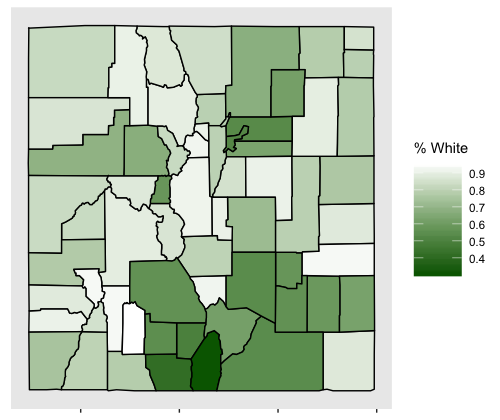
\includegraphics[width=0.8\linewidth]{/Users/tdounias/Desktop/Reed_Senior_Thesis/maps/pct_white_county_map} 

}

\caption{White voters per Colorado county}\label{fig:white pct map}
\end{figure}

Colorado is landlocked, and far from any coastal town; in place of
seaside resorts, Colorado attracts a substantial amount of tourists to
its mountains every year. They also heavily depend on federal money and
protection for national parks. Colorado has a median age of 34.3 and
median household income of \$65,685. Colorado's population is mostly
white, with a higher minority group population density in its Southern
regions, as shown in figure 3.1. {[}@us\_census\_bureau\_us\_2010{]}.
The conclusion here is that Colorado is a relatively young, mostly
white, and fairly well-off state that is increasingly getting more
diverse, particularly in the South. These factors are important as they
serve to associate Colorado with other states; such associations are
useful for the replication of this study or the generalization of my
results.

The State Capital is Denver; Colorado is split into 64 Counties, of
which the most populous are, in no particular order, the following: El
Paso, Denver, Arapahoe, Jefferson, Adams, Larimer, Boulder, and Douglas.
These counties comprise 73\% of the total population of Colorado.

\begin{longtable}[]{@{}lccl@{}}
\caption{Colorado population for largest counties
\label{tab:pop_table}}\tabularnewline
\toprule
\begin{minipage}[b]{0.13\columnwidth}\raggedright\strut
County\strut
\end{minipage} & \begin{minipage}[b]{0.21\columnwidth}\centering\strut
Total Population\strut
\end{minipage} & \begin{minipage}[b]{0.20\columnwidth}\centering\strut
CO Population \%\strut
\end{minipage} & \begin{minipage}[b]{0.34\columnwidth}\raggedright\strut
Largest Metro Area\strut
\end{minipage}\tabularnewline
\midrule
\endfirsthead
\toprule
\begin{minipage}[b]{0.13\columnwidth}\raggedright\strut
County\strut
\end{minipage} & \begin{minipage}[b]{0.21\columnwidth}\centering\strut
Total Population\strut
\end{minipage} & \begin{minipage}[b]{0.20\columnwidth}\centering\strut
CO Population \%\strut
\end{minipage} & \begin{minipage}[b]{0.34\columnwidth}\raggedright\strut
Largest Metro Area\strut
\end{minipage}\tabularnewline
\midrule
\endhead
\begin{minipage}[t]{0.13\columnwidth}\raggedright\strut
Adams\strut
\end{minipage} & \begin{minipage}[t]{0.21\columnwidth}\centering\strut
441603\strut
\end{minipage} & \begin{minipage}[t]{0.20\columnwidth}\centering\strut
0.08781\strut
\end{minipage} & \begin{minipage}[t]{0.34\columnwidth}\raggedright\strut
Denver-Aurora-Lakewood\strut
\end{minipage}\tabularnewline
\begin{minipage}[t]{0.13\columnwidth}\raggedright\strut
Arapahoe\strut
\end{minipage} & \begin{minipage}[t]{0.21\columnwidth}\centering\strut
572003\strut
\end{minipage} & \begin{minipage}[t]{0.20\columnwidth}\centering\strut
0.1137\strut
\end{minipage} & \begin{minipage}[t]{0.34\columnwidth}\raggedright\strut
Denver-Aurora-Lakewood\strut
\end{minipage}\tabularnewline
\begin{minipage}[t]{0.13\columnwidth}\raggedright\strut
Boulder\strut
\end{minipage} & \begin{minipage}[t]{0.21\columnwidth}\centering\strut
294567\strut
\end{minipage} & \begin{minipage}[t]{0.20\columnwidth}\centering\strut
0.05857\strut
\end{minipage} & \begin{minipage}[t]{0.34\columnwidth}\raggedright\strut
Boulder\strut
\end{minipage}\tabularnewline
\begin{minipage}[t]{0.13\columnwidth}\raggedright\strut
Denver\strut
\end{minipage} & \begin{minipage}[t]{0.21\columnwidth}\centering\strut
600158\strut
\end{minipage} & \begin{minipage}[t]{0.20\columnwidth}\centering\strut
0.1193\strut
\end{minipage} & \begin{minipage}[t]{0.34\columnwidth}\raggedright\strut
Denver\strut
\end{minipage}\tabularnewline
\begin{minipage}[t]{0.13\columnwidth}\raggedright\strut
Douglas\strut
\end{minipage} & \begin{minipage}[t]{0.21\columnwidth}\centering\strut
285465\strut
\end{minipage} & \begin{minipage}[t]{0.20\columnwidth}\centering\strut
0.05676\strut
\end{minipage} & \begin{minipage}[t]{0.34\columnwidth}\raggedright\strut
Denver-Aurora-Lakewood\strut
\end{minipage}\tabularnewline
\begin{minipage}[t]{0.13\columnwidth}\raggedright\strut
El Paso\strut
\end{minipage} & \begin{minipage}[t]{0.21\columnwidth}\centering\strut
622263\strut
\end{minipage} & \begin{minipage}[t]{0.20\columnwidth}\centering\strut
0.1237\strut
\end{minipage} & \begin{minipage}[t]{0.34\columnwidth}\raggedright\strut
Colorado Springs\strut
\end{minipage}\tabularnewline
\begin{minipage}[t]{0.13\columnwidth}\raggedright\strut
Jefferson\strut
\end{minipage} & \begin{minipage}[t]{0.21\columnwidth}\centering\strut
534543\strut
\end{minipage} & \begin{minipage}[t]{0.20\columnwidth}\centering\strut
0.1063\strut
\end{minipage} & \begin{minipage}[t]{0.34\columnwidth}\raggedright\strut
Denver-Aurora-Lakewood\strut
\end{minipage}\tabularnewline
\begin{minipage}[t]{0.13\columnwidth}\raggedright\strut
Larimer\strut
\end{minipage} & \begin{minipage}[t]{0.21\columnwidth}\centering\strut
299630\strut
\end{minipage} & \begin{minipage}[t]{0.20\columnwidth}\centering\strut
0.05958\strut
\end{minipage} & \begin{minipage}[t]{0.34\columnwidth}\raggedright\strut
Fort Collins\strut
\end{minipage}\tabularnewline
\begin{minipage}[t]{0.13\columnwidth}\raggedright\strut
Other\strut
\end{minipage} & \begin{minipage}[t]{0.21\columnwidth}\centering\strut
1378964\strut
\end{minipage} & \begin{minipage}[t]{0.20\columnwidth}\centering\strut
0.2742\strut
\end{minipage} & \begin{minipage}[t]{0.34\columnwidth}\raggedright\strut
\strut
\end{minipage}\tabularnewline
\begin{minipage}[t]{0.13\columnwidth}\raggedright\strut
Colorado\strut
\end{minipage} & \begin{minipage}[t]{0.21\columnwidth}\centering\strut
5029196\strut
\end{minipage} & \begin{minipage}[t]{0.20\columnwidth}\centering\strut
100\strut
\end{minipage} & \begin{minipage}[t]{0.34\columnwidth}\raggedright\strut
\strut
\end{minipage}\tabularnewline
\bottomrule
\end{longtable}

\clearpage

\subsubsection{The Politics of Colorado}\label{the-politics-of-colorado}

Curtis Martin (1962) notes that Colorado, due to its status as a
frontier state, has always been fiercely democratic and independent. He
connects this fact with Colorado's past, by pointing out that its
political institutions were deeply rooted in mining culture, ordinary
citizens' participation,a strong feeling of being ``far away'' from
sources of centralized power on the coasts, and a wish for the
protection and preservation of Colorado's natural environment. As such,
Colorado can be described as a populist state with a strong libertarian
streak, that highly values democratic processes when they serve the
people or protect and fund national parks, but staunchly opposes state
intervention when it is unwarranted{[}@martin\_colorado\_1962{]}.

This 1964 study of Colorado politics rings true to this day. One needs
not search for long to see instances when Colorado honored this
description. One example is TABOR, or the Taxpayer's Bill of Rights; a
strongly libertarian, small-government, populist series of regulations
that mandated a referendum for any measure that would increase state
taxes, and caped government spending. TABOR was passed by referendum in
1992, and later amended in 2005 after the dot com economic crisis
exposed the fact that inability to spend is very bad for a state
government trying to jump start its economy.
{[}@legislative\_council\_staff\_tabor\_2009{]}

Similarly, Amendment 64 passed in 2012 made Colorado one of the first
states to legalize the selling, possession, and consumption of
recreational marijuana; a policy advocated by progressives and
libertarians alike. Colorado was also the staging ground for what has
been coined the ``Sagebrush Rebellion'': a movement primarily consisting
of ranchers in dispute with the federal government over land use laws
and wildlife protection. While this ``rebellion'' primarily consisted of
battles in local legislatures or elections in the 1970s, its echoes can
be heard till today in events like the Bundy Standoff, with ranchers
taking up arms against federal employees and occupying federal land
{[}@thompson\_first\_2016{]}.

Setting policy aside, this description of Colorado is also confirmed by
polling data and election results. While being traditionally more
conservative, inflows of immigration from the South coupled with
increasing urban liberalization and tourism has led the state from
leaning republican to being aggressively purple: the quintessential
swing state. Colorado voted both for and later against Bill Clinton,
voted for G.W. Bush twice, and has supported democratic presidential
candidates since {[}@hamm\_how\_2017{]}. Additionally, when polled on
trust of federal or local governments, Colorado residents are
systematically skeptical; in a random sample poll conducted by Cronin
and Loevy (2012) in 2010, 56\% stated that their state officials were
lazy, wasteful, and inefficient. However--again indicating a
libertarian, independent streak--most Coloradoans from 1988 to today
consistently believe that their state is ``on the right track''
\footnote{Colorado College Citizens Polls, taken from Cronin et al.
  {[}@cronin\_colorado\_2012{]}}.

\subsubsection{Voting in Colorado}\label{voting-in-colorado}

Each County individually administers local, coordinated, primary, and
general elections, under the supervision of the Colorado Secretary of
State. This means that each county individually handles the voters
registered in that county. Unsurprisingly, the same eight most populous
counties are also the counties with the majority of registered voters,
as their registrants comprise 73\% of total Colorado registered voters
(as of November 2017). As table 3.2 shows, these eight counties have a
registration rate between 60-80\%, compared to a Colorado-wide rate of
about 67\%. Registration rates for all counties are also graphically
depicted in figure 3.2. In terms of Party registration, Colorado as a
whole leans democratic by a very narrow margin (figure 3.3).

\begin{longtable}[]{@{}lccc@{}}
\caption{Colorado voter registration for largest counties
\label{tab:voter_reg}}\tabularnewline
\toprule
\begin{minipage}[b]{0.10\columnwidth}\raggedright\strut
County\strut
\end{minipage} & \begin{minipage}[b]{0.24\columnwidth}\centering\strut
Total Registered Voters\strut
\end{minipage} & \begin{minipage}[b]{0.29\columnwidth}\centering\strut
County Registration Rate\strut
\end{minipage} & \begin{minipage}[b]{0.25\columnwidth}\centering\strut
\% of Statewide Registrants\strut
\end{minipage}\tabularnewline
\midrule
\endfirsthead
\toprule
\begin{minipage}[b]{0.10\columnwidth}\raggedright\strut
County\strut
\end{minipage} & \begin{minipage}[b]{0.24\columnwidth}\centering\strut
Total Registered Voters\strut
\end{minipage} & \begin{minipage}[b]{0.29\columnwidth}\centering\strut
County Registration Rate\strut
\end{minipage} & \begin{minipage}[b]{0.25\columnwidth}\centering\strut
\% of Statewide Registrants\strut
\end{minipage}\tabularnewline
\midrule
\endhead
\begin{minipage}[t]{0.10\columnwidth}\raggedright\strut
Adams\strut
\end{minipage} & \begin{minipage}[t]{0.24\columnwidth}\centering\strut
270,303\strut
\end{minipage} & \begin{minipage}[t]{0.29\columnwidth}\centering\strut
0.61\strut
\end{minipage} & \begin{minipage}[t]{0.25\columnwidth}\centering\strut
0.07\strut
\end{minipage}\tabularnewline
\begin{minipage}[t]{0.10\columnwidth}\raggedright\strut
Arapahoe\strut
\end{minipage} & \begin{minipage}[t]{0.24\columnwidth}\centering\strut
410,546\strut
\end{minipage} & \begin{minipage}[t]{0.29\columnwidth}\centering\strut
0.72\strut
\end{minipage} & \begin{minipage}[t]{0.25\columnwidth}\centering\strut
0.11\strut
\end{minipage}\tabularnewline
\begin{minipage}[t]{0.10\columnwidth}\raggedright\strut
Boulder\strut
\end{minipage} & \begin{minipage}[t]{0.24\columnwidth}\centering\strut
237,091\strut
\end{minipage} & \begin{minipage}[t]{0.29\columnwidth}\centering\strut
0.80\strut
\end{minipage} & \begin{minipage}[t]{0.25\columnwidth}\centering\strut
0.06\strut
\end{minipage}\tabularnewline
\begin{minipage}[t]{0.10\columnwidth}\raggedright\strut
Denver\strut
\end{minipage} & \begin{minipage}[t]{0.24\columnwidth}\centering\strut
450,616\strut
\end{minipage} & \begin{minipage}[t]{0.29\columnwidth}\centering\strut
0.75\strut
\end{minipage} & \begin{minipage}[t]{0.25\columnwidth}\centering\strut
0.12\strut
\end{minipage}\tabularnewline
\begin{minipage}[t]{0.10\columnwidth}\raggedright\strut
Douglas\strut
\end{minipage} & \begin{minipage}[t]{0.24\columnwidth}\centering\strut
237,659\strut
\end{minipage} & \begin{minipage}[t]{0.29\columnwidth}\centering\strut
0.83\strut
\end{minipage} & \begin{minipage}[t]{0.25\columnwidth}\centering\strut
0.06\strut
\end{minipage}\tabularnewline
\begin{minipage}[t]{0.10\columnwidth}\raggedright\strut
El Paso\strut
\end{minipage} & \begin{minipage}[t]{0.24\columnwidth}\centering\strut
445,708\strut
\end{minipage} & \begin{minipage}[t]{0.29\columnwidth}\centering\strut
0.71\strut
\end{minipage} & \begin{minipage}[t]{0.25\columnwidth}\centering\strut
0.12\strut
\end{minipage}\tabularnewline
\begin{minipage}[t]{0.10\columnwidth}\raggedright\strut
Jefferson\strut
\end{minipage} & \begin{minipage}[t]{0.24\columnwidth}\centering\strut
422,362\strut
\end{minipage} & \begin{minipage}[t]{0.29\columnwidth}\centering\strut
0.79\strut
\end{minipage} & \begin{minipage}[t]{0.25\columnwidth}\centering\strut
0.11\strut
\end{minipage}\tabularnewline
\begin{minipage}[t]{0.10\columnwidth}\raggedright\strut
Larimer\strut
\end{minipage} & \begin{minipage}[t]{0.24\columnwidth}\centering\strut
250,626\strut
\end{minipage} & \begin{minipage}[t]{0.29\columnwidth}\centering\strut
0.84\strut
\end{minipage} & \begin{minipage}[t]{0.25\columnwidth}\centering\strut
0.06\strut
\end{minipage}\tabularnewline
\begin{minipage}[t]{0.10\columnwidth}\raggedright\strut
Other\strut
\end{minipage} & \begin{minipage}[t]{0.24\columnwidth}\centering\strut
1,009,392\strut
\end{minipage} & \begin{minipage}[t]{0.29\columnwidth}\centering\strut
---\strut
\end{minipage} & \begin{minipage}[t]{0.25\columnwidth}\centering\strut
0.27\strut
\end{minipage}\tabularnewline
\begin{minipage}[t]{0.10\columnwidth}\raggedright\strut
Colorado\strut
\end{minipage} & \begin{minipage}[t]{0.24\columnwidth}\centering\strut
3,734,303\strut
\end{minipage} & \begin{minipage}[t]{0.29\columnwidth}\centering\strut
0.67\strut
\end{minipage} & \begin{minipage}[t]{0.25\columnwidth}\centering\strut
1.00\strut
\end{minipage}\tabularnewline
\bottomrule
\end{longtable}

\begin{figure}

{\centering 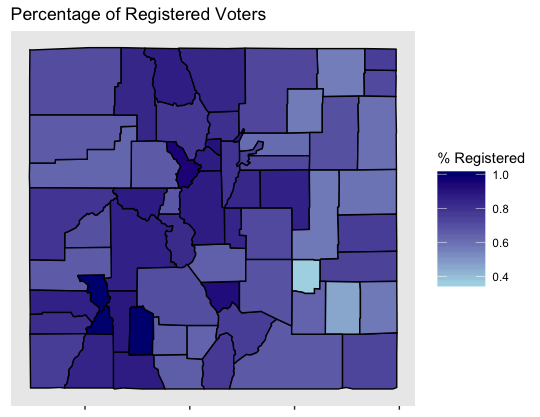
\includegraphics[width=0.8\linewidth]{/Users/tdounias/Desktop/Reed_Senior_Thesis/maps/pct_registered_county_map} 

}

\caption{Registration rates per Colorado county}\label{fig:reg per county map}
\end{figure}

\begin{figure}

{\centering 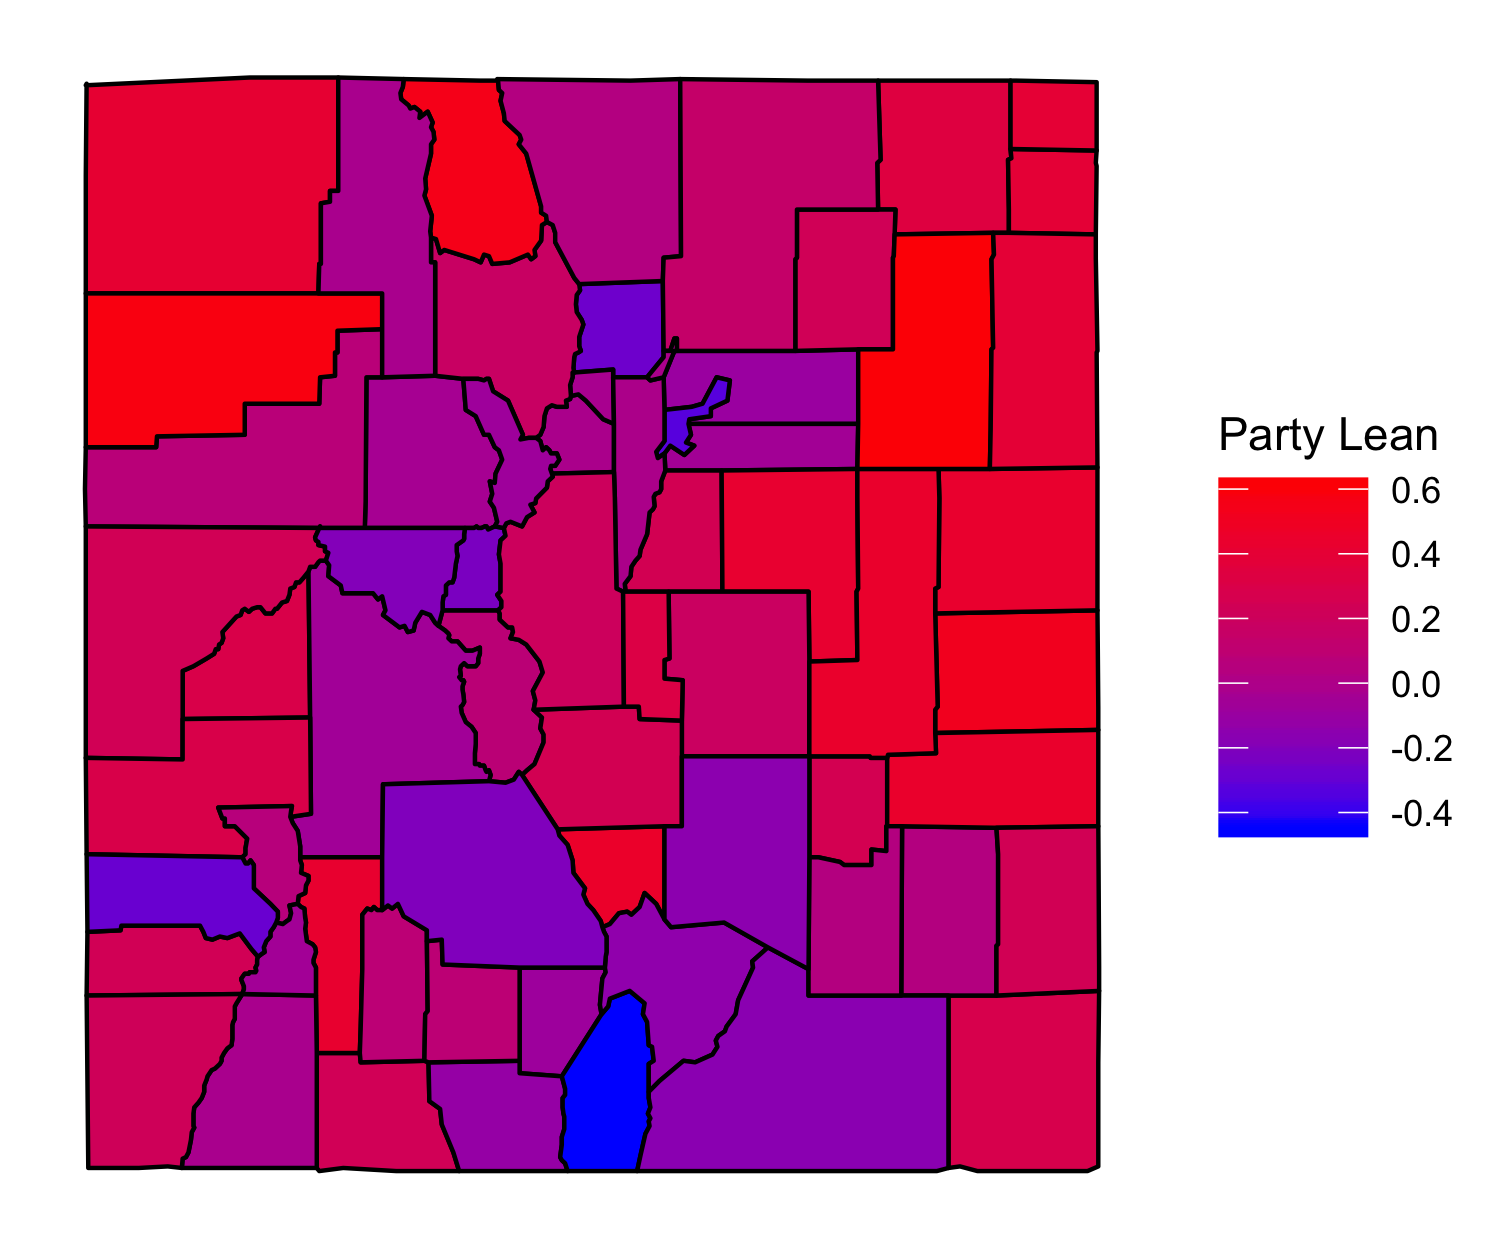
\includegraphics[width=0.8\linewidth]{/Users/tdounias/Desktop/Reed_Senior_Thesis/maps/party_affiliation_county_map} 

}

\caption{Democratic/Republican party lean per Colorado county}\label{fig:party reg per county map}
\end{figure}

In the past 25 years, there have been a series of key changes in the way
Colorado administers elections, in relation to Vote By Mail and other
reforms targeted and expanding the democratic franchise. In 1992,
Colorado introduced no-excuse absentee voting, allowing voters to either
physically pick up a mail ballot at a Vote Center or County Office, or
have a ballot mailed to them prior to election day. In 2008, this reform
was expanded to a permanent Vote-By-Mail system, which gave counties the
option to allow voters to be permanently put on a list of addresses that
received mail ballots prior to the election. The State also entered a
transitional status to full mail elections, giving counties the option
to make all coordinated local elections, general elections, and primary
elections exclusively VBM. In 2013, the Colorado State Legislature
passed HB13-1303: The Voter Access and Modernized Elections Act, which
mandated that every voter currently registered receive a mail ballot for
all future elections. The Act also expanded the use of Vote Centers
instead of traditional polling places, instituted same-day voter
registration, and revamped the way active and inactive voter status was
designated on voter rolls--more on this in future sections
{[}@hullinghorst\_voter\_2013{]}. These changes are summarized in Table
3.3.

\begin{longtable}[]{@{}cl@{}}
\caption{Key changes to Colorado elections policy
\label{tab:elect_policy}}\tabularnewline
\toprule
\begin{minipage}[b]{0.07\columnwidth}\centering\strut
Year\strut
\end{minipage} & \begin{minipage}[b]{0.87\columnwidth}\raggedright\strut
Key Changes\strut
\end{minipage}\tabularnewline
\midrule
\endfirsthead
\toprule
\begin{minipage}[b]{0.07\columnwidth}\centering\strut
Year\strut
\end{minipage} & \begin{minipage}[b]{0.87\columnwidth}\raggedright\strut
Key Changes\strut
\end{minipage}\tabularnewline
\midrule
\endhead
\begin{minipage}[t]{0.07\columnwidth}\centering\strut
1992\strut
\end{minipage} & \begin{minipage}[t]{0.87\columnwidth}\raggedright\strut
No Excuse Absentee Statewide Implementation\strut
\end{minipage}\tabularnewline
\begin{minipage}[t]{0.07\columnwidth}\centering\strut
2008\strut
\end{minipage} & \begin{minipage}[t]{0.87\columnwidth}\raggedright\strut
Permanent No-Excuse VBM Lists, Option of Full-VBM Elections\strut
\end{minipage}\tabularnewline
\begin{minipage}[t]{0.07\columnwidth}\centering\strut
2013\strut
\end{minipage} & \begin{minipage}[t]{0.87\columnwidth}\raggedright\strut
Automatic Mail Ballot System Implemented Statewide, Established Vote
Centers\strut
\end{minipage}\tabularnewline
\bottomrule
\end{longtable}

\subsubsection{Colorado as a Case for this
Thesis}\label{colorado-as-a-case-for-this-thesis}

Colorado presents such an interesting case for research on Vote By Mail
exactly because it has gone through such a long transitional process to
reach its current elections system. It has steadily developed voting
policy through a mixture of state mandates, county action, and outside
policy motivations. Colorado's streak of independence and direct
democracy is also very apparent in this shift in electoral practices,
since they have been passing policies trying to expand participation for
a very long time. It gives researchers access to approximately 22 years
during which at least part of the state conducted elections by mail,
making comparative, county- or individual-level case studies
particularly alluring. Colorado's streak of independence and direct
democracy is also very apparent in this shift in electoral practices,
since they have been passing policies trying to expand participation for
a very long time.

On a more general level, Colorado is interesting exactly because it is
``typical'' but with a wild streak. It is typical rocky mountain
country, great planes country, and liberal urban city but all \emph{in
one state}. In is libertarian yet increasingly Democratic. It heavily
relies on state funding for national parks, yet rebels against federal
land use laws. It is a frontier state with traditional values, that
overwhelmingly supports marijuana legalization. It is also a consistent
purple state, with a Democratic Governor and House, but Republican
Attorney General, Secretary of State and Senate. This means that
Colorado is a combination of distinct national effects, but also local
effects that make it significantly different from national trends as a
whole. In this environment, predicting results of policy can be
difficult, but extremely salient as multiple effects can be tested
against each other.

\subsection{The Data}\label{the-data}

This thesis relies on county and individual level models to draw
conclusions on voting behaviors, and how they are affected by voting
method. As such, the data I need will optimally contain the following:

\begin{itemize}
\item
  \textbf{County and individual level demographic characteristics}:
  race, gender, urban population
\item
  \textbf{County and individual level voting data}: turnout, party
  registration, total registrants
\item
  \textbf{Information on individual elections}: date, ballots cast,
  voting methods, county, election descriptions
\end{itemize}

In the process of my research, I have acquired sufficient data to cover
the second and third of these areas. I was unable to procure individual
level data on demographic characteristics apart from gender, age, and
party registration. Reasonable conclusions can still be drawn from
county or precinct aggregates.

\subsubsection{Sources and first glance}\label{sources-and-first-glance}

I used two sources of data: Colorado voter records gathered by the
Colorado Secretary of State's office, and demographic data from the 2010
US Census. In the process of procuring these data I was aided by a
series of other researchers and professionals with experience in the
field of elections administration. Andrew Menger, Postdoctoral Fellow at
the Weidenbaum Center on the Economy, Government, and Public Policy at
Washington University, was kind enough to give me access to data files
for Colorado for the years of 2012-2016 that he had already collected
for his research\footnote{Doctor Menger's website with links to his
  research can be found at www.andrewmenger.com}. I directly obtained
the 2017 from the Colorado Secretary of State's office, with the help of
Mr.~Judd Choate, Director of Elections.

\paragraph{2010 US Census}\label{us-census}

The US Census is conducted country-wide every ten years, with the goal
of procuring accurate data on the demographic characteristics of the
population. The Census uses a combination of federal field workers
conducting door-to-door canvassing and statistical methods for data
aggregation. From the 2010 Census, which is publicly available online, I
get total population counts, characteristics on race, and rural/urban
population counts for Colorado.

I use two datasets from the Census. For both, the unit of observation is
one of the 64 counties of Colorado, and both include the same total
population counts. One contains racial demographic characteristics and
the other contain percentages of rural and urban populations in each
county. The racial demographic dataset needed some wrangling work to
extract a percentage of white residents in each county. Individuals were
coded as ``white'' when they identified as exclusively white--this
doesn't include mixed-race individuals reporting white ancestry.

\paragraph{Colorado Voter Files}\label{colorado-voter-files}

As mandated by HAVA, Colorado maintains a statewide registry of all
currently registered voters. This registry is typically under the
purview of the Secretary of State. Voter Registration Files are
constantly updated with new information on existing voters, new voters,
or with the removal of inactive or otherwise ineligible voters.
Therefore, this file will be different every time it is accessed or
shared. Based on when this file is accessed, only a ``snapshot'' of the
file can be obtained. Similarly with VRFs, a Voter History File is
maintained and constantly updated by the state. This file is uniquely
connected to its VRF: only voters showing up as registrants will have
their histories included. I have both Voter Registration and History
files for the years between 2012-2017, obtained with the help of Judd
Choate and Andrew Menger.

In the Voter Registration files, the unit of observation is the
individual voter, and all variables are initially coded as character
strings. Each voter is assigned a unique voter ID, which serves as a
point of reference between the two files. Broadly speaking, data in this
file can be divided between three categories: first, personal
identification information like address, ZIP code, or phone number;
second, demographic information like age and gender; third, information
pertinent to elections administration like congressional district, local
elections for which the individual should receive a ballot, voter ID,
and party registration. I will further elaborate on relevant variables
in the wrangling section.

In the Voter History files, the unit of observation here is a single
ballot cast, and all variables are initially coded as character strings.
This means that for each voter registered--and so included in the
VRF--the history file should contain an observation for each time they
voted. This file includes two types of data: first, identifiers for the
election like county, date, description, and type; second, identifiers
for the individual vote including voter ID and voting method.

\subsubsection{Why Voter Registration
Files?}\label{why-voter-registration-files}

Voter Registration and History files are suitable sources for my
analysis because they contain all the data that is necessary for a first
pass at testing my hypotheses: voting method, county, election level,
active registration, registration dates, and a series of individual
characteristics like party registration, age, or gender. These data, and
the demographic data in particular, are also in the most basic unit of
observation: the ballot level\footnote{A good heuristic for what
  ``ballot'' level means is a specific individual at the time when they
  cast a specific ballot. Between ballots all characteristics may
  change: age, gender, party registration etc., which is why the
  ``ballot'' level is distinct from the individual level.}. This means
that I do not need to establish any process to infer individual
characteristics from population-wide statistics.

In statistical science, sampling is the process by which individual
units are selected from a population. The sample selected should be
\emph{representative} of the whole so that it can be used to infer
characteristics of the general population. Despite a vast array of
techniques to ensure that sampling is representative, there is always
room for error. Voter Registration Files are an excellent source of data
because they do not involve any sampling whatsoever; they include
\emph{all} currently registered voters and voter histories. This
characteristic helps cut down on data-related errors and on the
complexity of data extraction.

An additional characteristic of these data is that they are concentrated
and relatively uniform. Data transfer errors still exist, and the
wrangling process is never entirely straightforward. Still, the data are
almost completely uniform in how variables are encoded. Over thirty five
million observations are included in my final, cumulative voter history
dataset, and all of them have, for example, the same types of entry for
party registration (REP, DEM, UAF etc.). Admittedly, this may just be a
characteristic of the Colorado files, since they are the only ones I
used for my research.

A last benefit of using Voter Registration Files comes from the
replicability they allow for. These files are generally public, with
access to them including only data transfer and administrative costs.
This makes peer-review and replication less complicated than if, say, I
was using private survey data. It also allows for expansion that goes
beyond the State of Colorado; my code can be adapted to fit different
data, making future comparative studies more likely and less
time-consuming than starting from scratch.

\subsection{Wrangling the Data}\label{wrangling-the-data}

The process of ``wrangling'' refers to manipulating the data into a form
that can then be used for graphing, exploratory data analysis,
modelling, or presentation. In this case, wrangling also included
aggregating data across multiple sources and datasets. For this purpose,
I made heavy use of the \texttt{tidyverse} \textit{R} package, and in
particular the \texttt{dplyr} package. In this section I will go through
some of the key problems encountered during the wrangling of these data,
and then discuss the final form each variable takes.

\subsubsection{Initial Problems with the 2017 Voter File and
Solution}\label{initial-problems-with-the-2017-voter-file-and-solution}

In my initial research I intended to only use the 2017 snapshots of the
Colorado Registration and History file. The major issue I encountered,
which merits discussion in its own section, comes from the fact that the
records I have access to are ``snapshots''. What this means, is that for
each person in each year of voter registration files, I have their
corresponding history files for all ballots they have cast in Colorado,
but not their own history of registration and migration. If, say, a
voter moved from Boulder County to Summit County, I would have their
votes in Boulder County show up in the voter history file, but them
being registered in Summit. If you recall the turnout calculations
specified earlier on, this implies an overestimation when looking back
at elections that happened some time before the date of the
``snapshot''. Additionally, ``snapshots'' of current voter files do not
reflect voters dropping off the rolls for whatever reason (death, moving
out of the state, long term inactivity, non-confirmable personal data
etc.)

After going through turnout calculations with the 2017 files, a
significant majority of counties appeared to have turnout exceeding
80\%, particularly for years between 2000 and 2012. This was, to put it
mildly, concerning. With the aforementioned help, I was given access to
similar ``snapshots'' for each year between 2012-2016. After similar
calculations, I returned figure 3.4 for the eight most populous counties
as described above, including different shapes for election type, colors
for county, and a vertical line at 2013 to signify the latest major
change in how Colorado administers elections.

\begin{figure}

{\centering 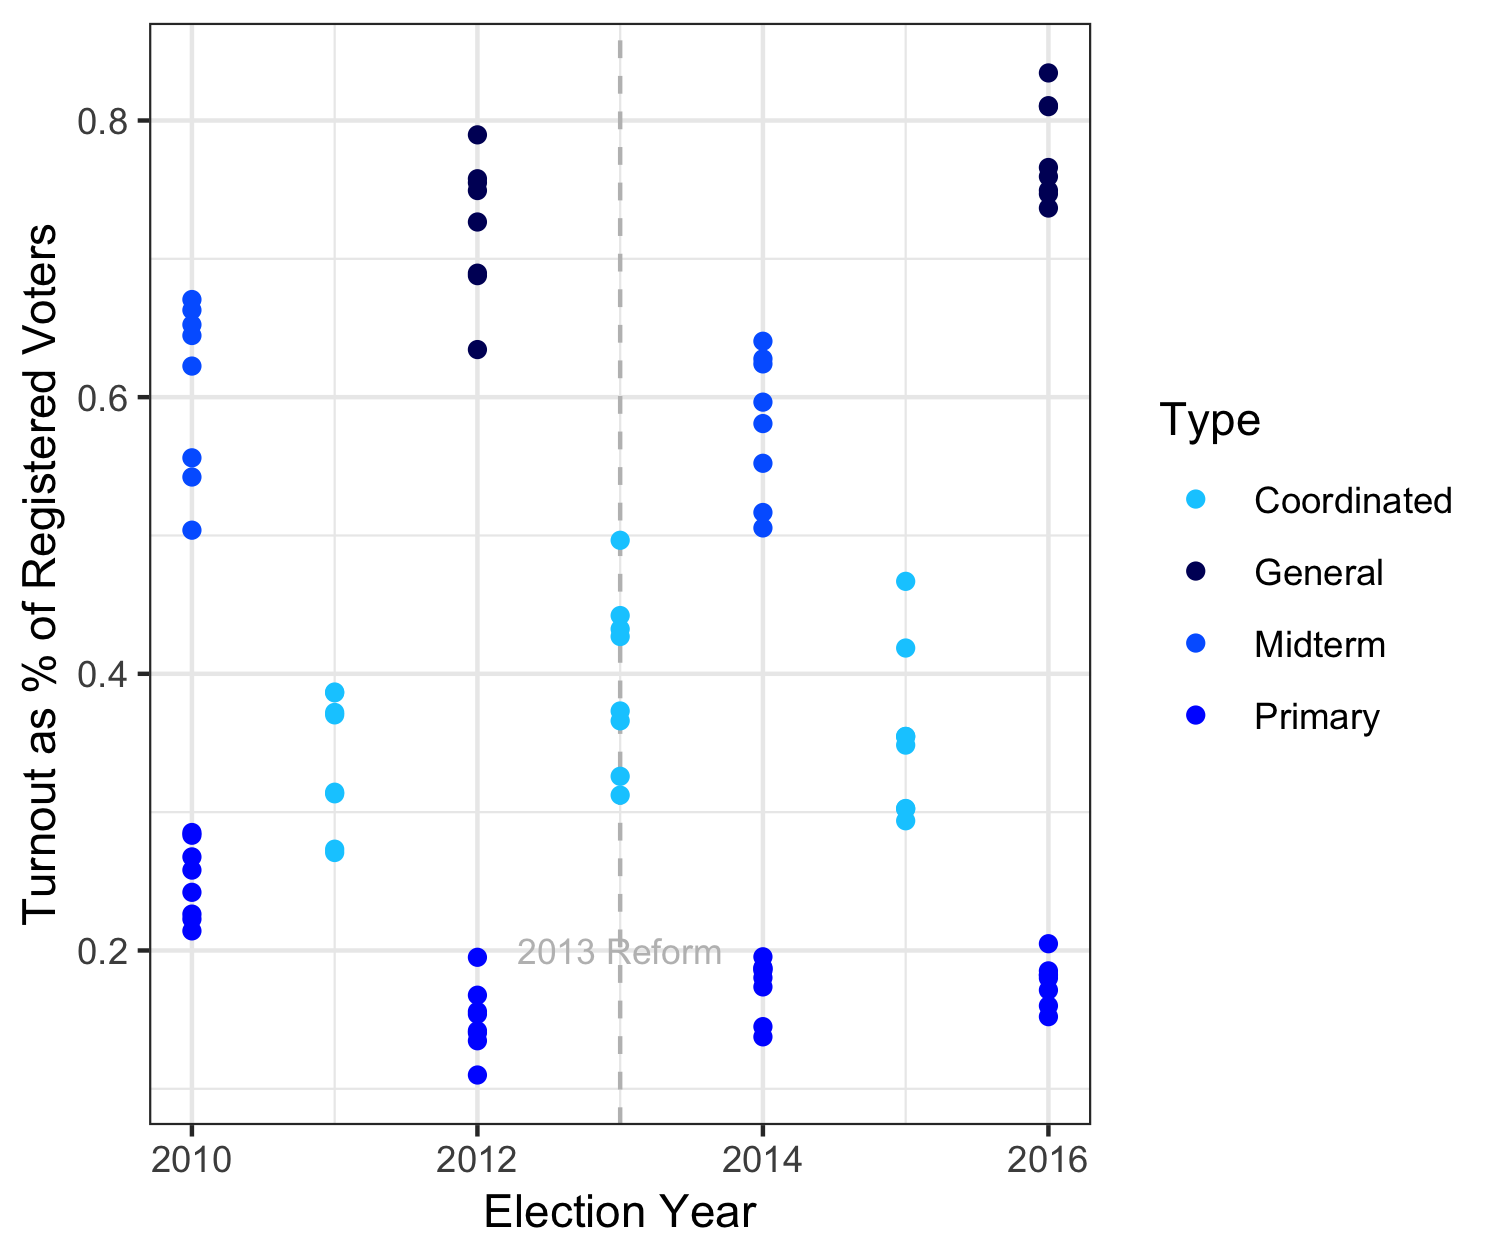
\includegraphics[width=0.8\linewidth]{/Users/tdounias/Desktop/Reed_Senior_Thesis/plots/colorado_bigeight_turnout_graph} 

}

\caption{Turnout plot for eight largest Colorado counties, 2012-2016}\label{fig:big eight turnout plot}
\end{figure}

To also further illustrate the in-county migration and dropped voter
problem, I created a graph that includes logged total counts of
registered voters calculated using the 2017 and the 2012-2016 files. The
plot also includes a line at \(y = x\). If in-Colorado migration and
dropped voters are not an issue, most points on this graph should be at
this line.

\begin{figure}

{\centering 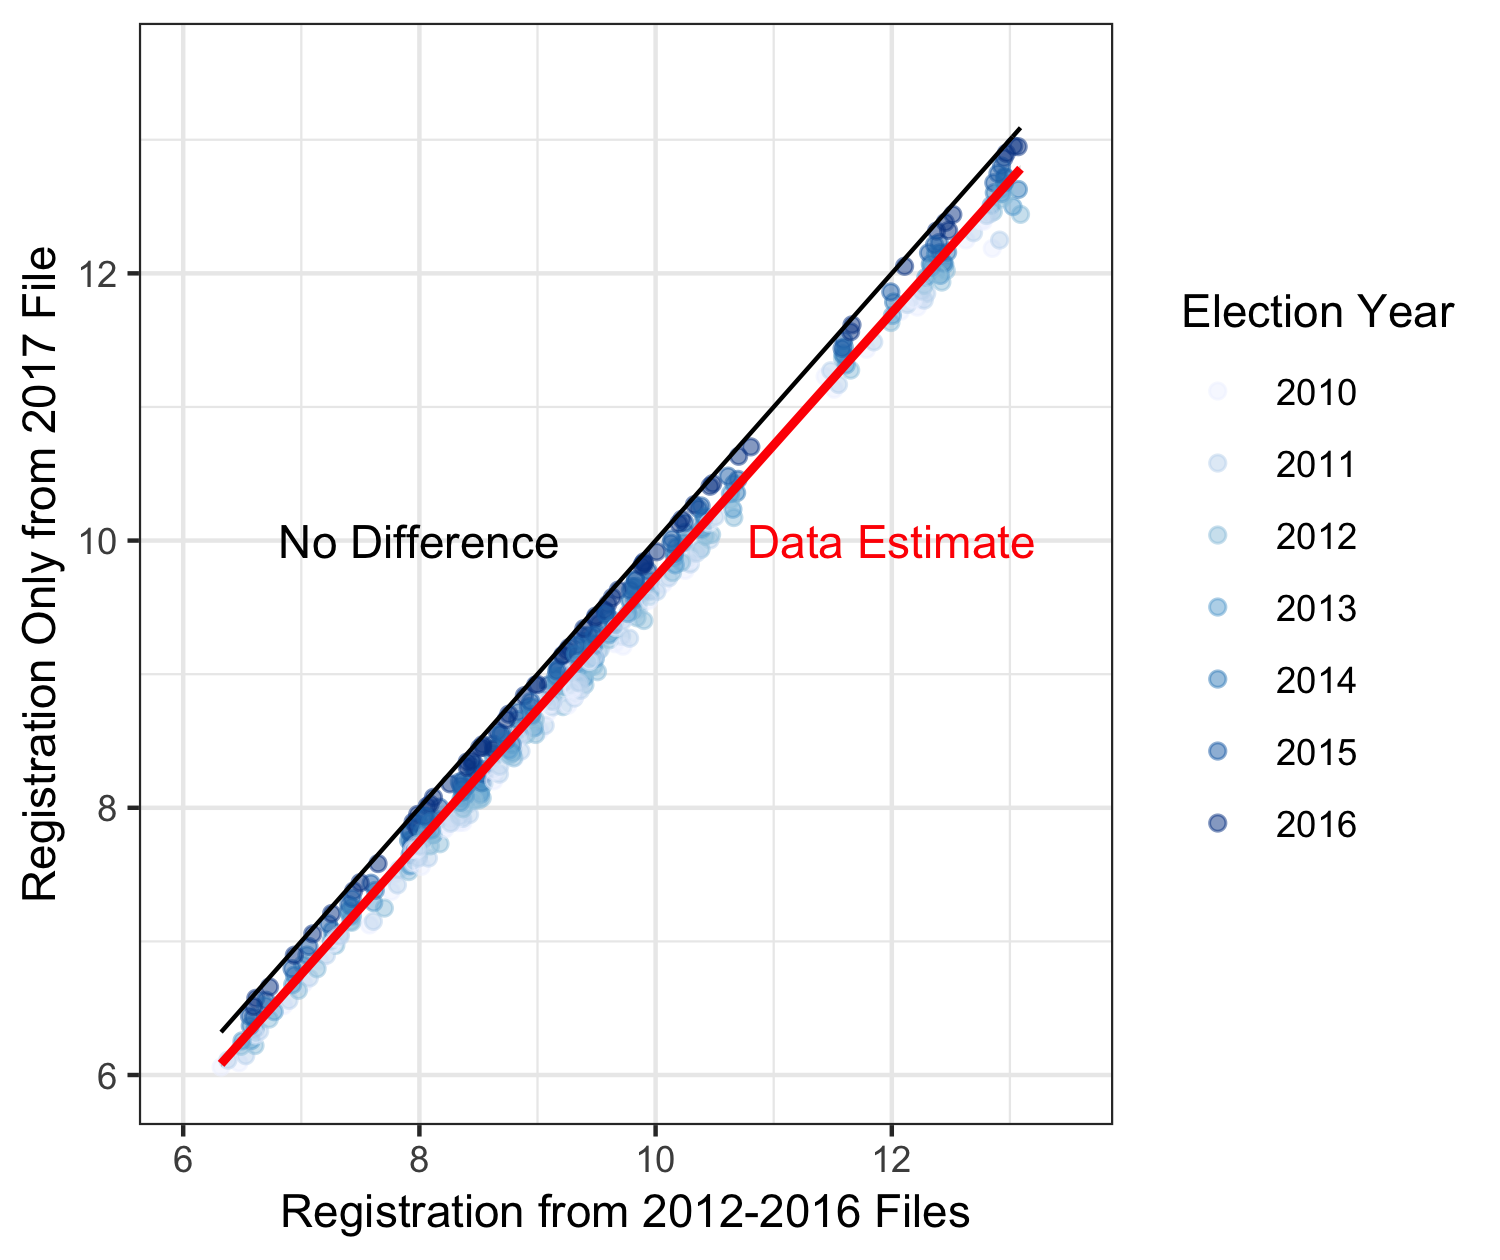
\includegraphics[width=0.8\linewidth]{/Users/tdounias/Desktop/Reed_Senior_Thesis/plots/county_migration_A} 

}

\caption{Comparison of registration count methods}\label{fig:county migration A}
\end{figure}

Two things should be clear from figure 3.5. First, there is significant
deviation between the counts using just the 2017 file and all files
across years. Specifically, the 2017 count consistently underestimates
the total amount of registered voters--this is shown by the red linear
model smoothing line. This consistent difference means that it is close
to impossible to generate safe conclusions on my hypotheses using only
the 2017 files and the methods I have outlined in Chapter 2. Second,
counts get more accurate the closer to 2017 we get. This should be even
more apparent in figure 3.6, which limits the scale to only some high
registration counties, and adds a shape indicator for county.

\begin{figure}

{\centering 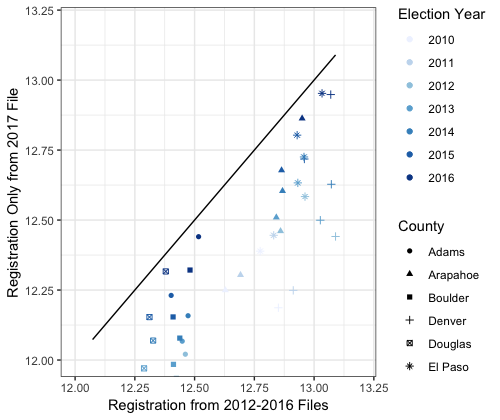
\includegraphics[width=0.8\linewidth]{/Users/tdounias/Desktop/Reed_Senior_Thesis/plots/county_migration_B} 

}

\caption{Comparison of registration count methods only for a few counties, 2012-2016}\label{fig:county migration B}
\end{figure}

Here the structure of the data becomes clear: for each county, there are
a series of almost vertically distributed points, which get closer to
the \(y=x\) line the closer the counts get to 2017. Through this series
of tests, it became clear that using multiple years of data was
necessary in order to conduct an accurate test of my hypotheses. My
selection was later vindicated, when looking at comparisons between
reported rates of turnout\footnote{Turnout is calculated over all
  registered voters} and turnout calculated through my dataset for the
2014 midterm election (see fig. 3.7).

\begin{figure}

{\centering 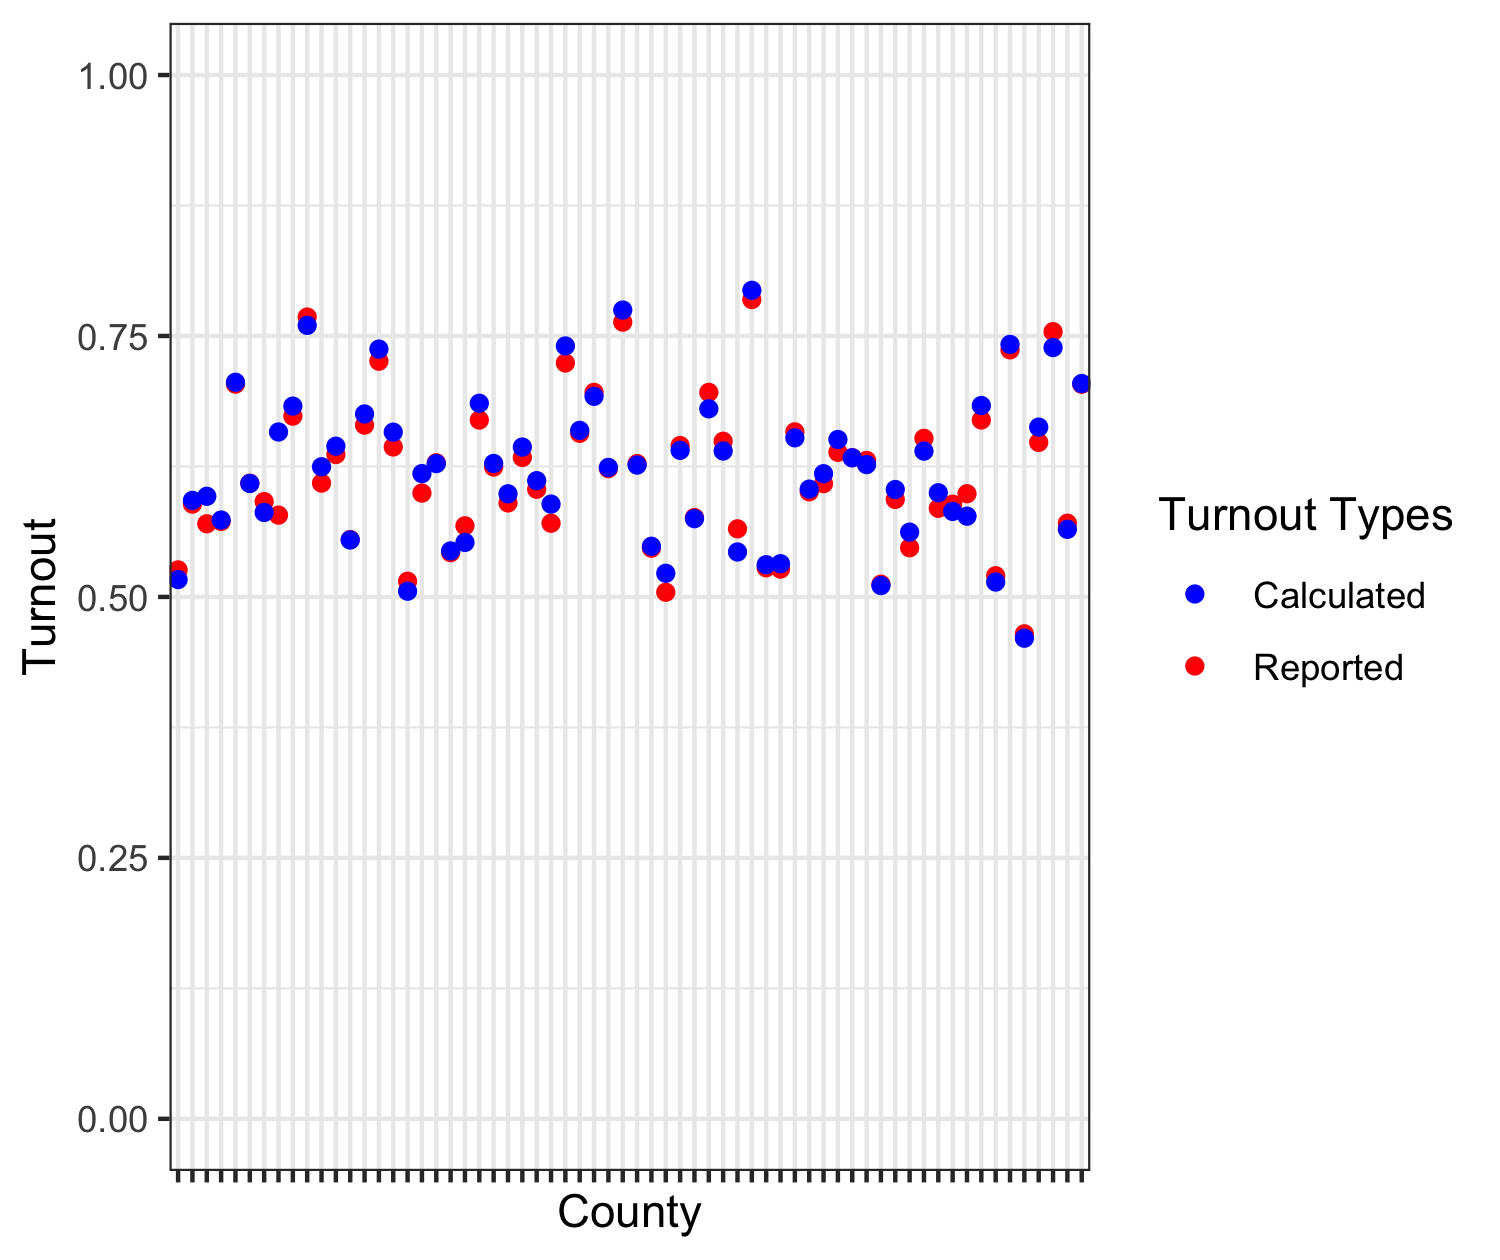
\includegraphics[width=0.8\linewidth]{/Users/tdounias/Desktop/Reed_Senior_Thesis/plots/Calc_vs_rep_turnout} 

}

\caption{Comparison of reported and calculated turnout for 2014 midterms across county}\label{fig:comp turnout 2014}
\end{figure}

The differences are insignificant. They exist because of ``noise'' added
on because of errors in the data, misreporting, registration records
redacted due to privacy concerns, voters dropped before the ``snapshot''
occurred, and other similar factors.

\subsubsection{Other Wrangling Issues}\label{other-wrangling-issues}

Wrangling the data was the majority of the work that went into this
thesis. As will become clear in this section, apart from accurately
processing, diagnosing, and merging the data, the process of wrangling
includes several non-trivial decisions about how to treat missing values
and variable specification. Including a full account would probably read
like the world's most cliche crime novel: a series of elusive final
datasets, a plucky yet occasionally naive young detective, two wisened
mentors, clues, dead ends, frustration, compromise,
and\ldots{}spreadsheets. I will spare the reader the whole story, but I
will include a non-comprehensive list of some of the difficulties
associated with wrangling voter files, as it was a crucial part of the
learning process I underwent while doing my research.

\textbf{Missing Values}: The decision on how to deal with missing
values--or NAs--in a dataset is a lot more important than it may
initially seem. A first, intuitive reaction might be to just disregard
them; however this works under the assumption that there is no structure
inherent to why these data are missing. To give just two examples, in
the data I have collected the PARTY value for the 2015 voter
registration file is missing. If I excluded all observations with
missing PARTY values, I would be excluding a fifth of my data. Missing
values were also present in the VOTING\_METHOD variable of the voter
history files. While this may have seemed troubling, after closer
examination it was revealed that the vast majority of such missing
values was concentrated in Jefferson County, and in elections prior to
2002. Therefore, these observations could be ignored, since they played
no role in my final dataset. The conclusion should be that choices made
on exclusion, inclusion, or estimation of missing data are very
important, and should be taken with much care and consideration for the
underlying structure of the data.

\textbf{Data Input Errors}: Is ``QATAR'' a political party in Colorado?
State records say not. However, ``QATAR'' did show up as a value for the
Party variable for my 2016 voter registration file snapshot. This may
occur for a number of reasons, the most likely of which is the
introduction of errors when transferring these data. The data have been
read and written by multiple operating systems (iOS and Windows) and
programming platforms (STATA, R); they have also been uploaded,
downloaded, and written unto CDs, as well as transferred between County
and Colorado Secretary of State's Office when they were created.
Characters that would be normally read into one platform as line or
value delimiters may have been misinterpreted by another platform, with
no operator error involved. In my analysis I treated all values that
seemed more likely than not to be errors as NAs. There were not many of
these--less than \(.001%\) of my data--but they were a hassle to find,
analyze, and then recode into some useful value.

\textbf{Data Size}: Nothing to write home about here, just an
observation that multiple voter registration files can be \emph{huge},
which puts considerable strain on a computer's processing power. This
means that wrangling has to comprise of a series of careful, deliberate
moves. Brute force should be discouraged, as a dead end means several
hours of melodic computer fan panic.

\textbf{Joining, Merging, Spreading, and the Multiplicity of Levels}:
For the data to end up in any functional shape, it eventually becomes
necessary to start joining datasets. Thankfully, a clear division of
modelling tasks between county and individual level models means that
joining on COUNTY or VOTER\_ID is ideal, and fairly straightforward. As
will become clear in later sections, I also had to consider the variety
of different units of observation, specifically: county, individual,
ballot, election, county-by-election.

\subsubsection{Final Variable
Specifications}\label{final-variable-specifications}

After the conclusion of the wrangling process, the resulting dataset
included a series of discrete and continuous variables. I will briefly
outline them here, along with their range and values.

\begin{itemize}
\tightlist
\item
  VOTER\_ID: Discrete variable, unique value given to each individual
  voter. Useful for merging.
\item
  COUNTY: Discrete variable, the 64 counties of Colorado.
\item
  REGISTRATION\_DATE: Discrete variable, date of registration for each
  registrant. Useful to get total registrants on election day.
\item
  TURNOUT: Continuous variable, in the range {[}0,1{]}. The response
  variable for my county-level models.
\item
  ELECTION\_TYPE: Discrete variable, the four types of elections:
  Primary, Coordinated, Midterm, Presidential.
\item
  ELECTION\_DATE: Discrete variable, self-explanatory.
\item
  VBM\_PCT: Continuous variable, in the range {[}0,1{]}. This is the
  focus of my analysis, as it counts the percentage of total ballots
  that were mail ballots.
\item
  PCT\_WHITE: Continuous variable, in the range {[}0,1{]}. Percentage of
  white residents per county.
\item
  PCT\_URBAN: Continuous variable, in the range {[}0,1{]}. Percentage of
  urban residents per county.
\item
  PARTY: Discrete variable. For each voter, the party they are
  registered with. Can be: Republican, Democrat, Other, or Unaffiliated.
\item
  GENDER: Discrete binary variable, Male or Female.
\item
  AGE: The age of the individual registrant.
\item
  VOTING\_METHOD: The method used by an individual voter to cast their
  ballot. Is coded as either VBM or In Person, according to Table 3.4:
\end{itemize}

\begin{longtable}[]{@{}lll@{}}
\caption{Voting methods coding table
\label{tab:voting_methods_table}}\tabularnewline
\toprule
\begin{minipage}[b]{0.22\columnwidth}\raggedright\strut
Voting Method\strut
\end{minipage} & \begin{minipage}[b]{0.42\columnwidth}\raggedright\strut
Description of Method\strut
\end{minipage} & \begin{minipage}[b]{0.18\columnwidth}\raggedright\strut
Designation\strut
\end{minipage}\tabularnewline
\midrule
\endfirsthead
\toprule
\begin{minipage}[b]{0.22\columnwidth}\raggedright\strut
Voting Method\strut
\end{minipage} & \begin{minipage}[b]{0.42\columnwidth}\raggedright\strut
Description of Method\strut
\end{minipage} & \begin{minipage}[b]{0.18\columnwidth}\raggedright\strut
Designation\strut
\end{minipage}\tabularnewline
\midrule
\endhead
\begin{minipage}[t]{0.22\columnwidth}\raggedright\strut
Absentee Carry\strut
\end{minipage} & \begin{minipage}[t]{0.42\columnwidth}\raggedright\strut
Voters who carried an absentee ballot with them from an early voting
location or county office\strut
\end{minipage} & \begin{minipage}[t]{0.18\columnwidth}\raggedright\strut
VBM\strut
\end{minipage}\tabularnewline
\begin{minipage}[t]{0.22\columnwidth}\raggedright\strut
Absentee Mail\strut
\end{minipage} & \begin{minipage}[t]{0.42\columnwidth}\raggedright\strut
Voters who were sent an absentee ballot, and mailed it in\strut
\end{minipage} & \begin{minipage}[t]{0.18\columnwidth}\raggedright\strut
VBM\strut
\end{minipage}\tabularnewline
\begin{minipage}[t]{0.22\columnwidth}\raggedright\strut
Early Voting\strut
\end{minipage} & \begin{minipage}[t]{0.42\columnwidth}\raggedright\strut
Voters who physically went to an Early Voting location and voted\strut
\end{minipage} & \begin{minipage}[t]{0.18\columnwidth}\raggedright\strut
In Person\strut
\end{minipage}\tabularnewline
\begin{minipage}[t]{0.22\columnwidth}\raggedright\strut
In Person\strut
\end{minipage} & \begin{minipage}[t]{0.42\columnwidth}\raggedright\strut
Voters who physically went to a polling place and voted on paper\strut
\end{minipage} & \begin{minipage}[t]{0.18\columnwidth}\raggedright\strut
In Person\strut
\end{minipage}\tabularnewline
\begin{minipage}[t]{0.22\columnwidth}\raggedright\strut
Mail Ballot\strut
\end{minipage} & \begin{minipage}[t]{0.42\columnwidth}\raggedright\strut
Vote By Mail\strut
\end{minipage} & \begin{minipage}[t]{0.18\columnwidth}\raggedright\strut
VBM\strut
\end{minipage}\tabularnewline
\begin{minipage}[t]{0.22\columnwidth}\raggedright\strut
Polling Place\strut
\end{minipage} & \begin{minipage}[t]{0.42\columnwidth}\raggedright\strut
Traditional polling place voting, discontinued in 2013\strut
\end{minipage} & \begin{minipage}[t]{0.18\columnwidth}\raggedright\strut
In Person\strut
\end{minipage}\tabularnewline
\begin{minipage}[t]{0.22\columnwidth}\raggedright\strut
Vote Center\strut
\end{minipage} & \begin{minipage}[t]{0.42\columnwidth}\raggedright\strut
Voters who cast their ballots at Vote Centers\strut
\end{minipage} & \begin{minipage}[t]{0.18\columnwidth}\raggedright\strut
In Person\strut
\end{minipage}\tabularnewline
\bottomrule
\end{longtable}


\end{document}
